\documentclass[preprint,10pt,3p]{elsarticle}
\usepackage{ecrc}
\volume{00}
\firstpage{1}
\journalname{Expert Systems with Applications}
\runauth{}
\jid{ExpertSystAppl}
\jnltitlelogo{}
\CopyrightLine{2011}{Published by Elsevier Ltd.}
\usepackage{xcolor}
\usepackage{amssymb}
\usepackage{pdfpages}
\usepackage[figuresright]{rotating}
\usepackage{lscape}
\usepackage{multirow}
\usepackage{graphicx}
\usepackage{amssymb,amsmath}
\usepackage{lineno}
\usepackage{setspace}
\usepackage{graphicx}
\usepackage{epsfig}
\usepackage{multirow}
\usepackage{twcal}
\usepackage{relsize}
\usepackage{array}
\usepackage{booktabs}
\usepackage[linesnumbered,vlined,boxed]{algorithm2e}
\usepackage{amssymb}
\usepackage{tabularx,multirow,booktabs}
\usepackage{amsthm}
\usepackage[T1]{fontenc}
\usepackage{textcomp}
\usepackage{url}
\usepackage[figuresright]{rotating}
\usepackage[breaklinks=false]{hyperref}
\usepackage{ragged2e}

\newcommand{\tab}[1]{\hspace{.25 \textwidth}\rlap{#1}}
\bibliographystyle{abbrvnat}

\setcitestyle{authoryear,round, sort&compress}
\biboptions{semicolon}

\hypersetup{
     colorlinks   = true,
     citecolor    = blue
}

\usepackage{lmodern}
\usepackage[utf8x]{inputenc}

\definecolor{airforceblue}{rgb}{0.36, 0.54, 0.66}
\definecolor{alizarin}{rgb}{0.82, 0.1, 0.26}
\definecolor{amber}{rgb}{1.0, 0.75, 0.0}
\definecolor{amethyst}{rgb}{0.9, 0.5, 0.9}
\definecolor{ao}{rgb}{0.0, 0.0, 1.0}
\definecolor{ao(english)}{rgb}{0.0, 0.5, 0.0}
\definecolor{atomictangerine}{rgb}{1.0, 0.6, 0.4}
\definecolor{azure(colorwheel)}{rgb}{0.0, 0.5, 1.0}
\definecolor{bittersweet}{rgb}{1.0, 0.44, 0.37}
\definecolor{bluebell}{rgb}{0.14, 0.24, 0.82}
\definecolor{psychedelicpurple}{rgb}{0.87, 0.0, 1.0}
\definecolor{ultramarine}{rgb}{0.07, 0.04, 0.56}
\definecolor{armygreen}{rgb}{0.29, 0.33, 0.13}

\usepackage{chngcntr}
\counterwithout{figure}{section}
\counterwithout{figure}{subsection}
\counterwithout{table}{section}
\counterwithout{table}{subsection}

\usepackage{amsmath}
\usepackage{amssymb}
\usepackage{mathtools,amssymb,lipsum}
\usepackage[symbol]{footmisc}
\usepackage{lipsum}
\usepackage{mathtools}
\usepackage{makeidx}
\usepackage{multirow}
\usepackage{multicol}
\usepackage{xcolor}


\begin{document}



\begin{frontmatter}

\author{Pinar Civicioglu\fnref{label1}}
\ead{civici@erciyes.edu.tr}
\address{Erciyes University, Faculty of Aeronautics and Astronautics, Dept. of Aircraft Electrics and Electronics, Kayseri, Turkey\fnref{label2}}
\author{Erkan Besdok\corref{cor1} \fnref{label2}}
\ead{ebesdok@erciyes.edu.tr}
\address{Erciyes University, Faculty of Engineering, Dept. of Geomatics Eng., Kayseri, Turkey\fnref{label2}}
\fntext[label1]{Tel.: +xxx-xx fax: +xxx-xx.}
\cortext[cor1]{Corresponding author}
\fntext[label2]{Tel.: +xxx-xx; fax: +xxx-xxx.}

\title{Bernstain-Search Differential Evolution Algorithm :  BSD }

\end{frontmatter}



\section{Cite As ;}
\label{sec:01}
$Civicioglu, P., Besdok, E.$, (2019), Bernstain-search differential evolution algorithm for numerical function optimization,  Expert Systems with Applications, 138 (30), 112831\\
\\
\\
Terminology ;\\
"Bernstain polynomials" \citep{30} == "Bernstein polynomials" \citep{40}\\
\\
\\

\section{Bernstain-Search Differential Evolution Algorithm : BSD}
\label{sec:02}
\par
In the literature of evolutionary algorithms, a random solution is called a \emph{pattern vector} and N \emph{pattern vectors} form the \emph{pattern matrix} P. Each \emph{pattern vector} consists of D \emph{individual}s. EAs can perform \emph{bounded} and/or \emph{unbounded} search. Bounded search works between the upper and lower limits of the individuals \citep{5,6,7,29}. \textcolor{bluebell}{BSD} is designed as a global minimizer algorithm that performs bounded search.

In \textcolor{bluebell}{BSD}, individuals are determined using Eq~\ref{eq1};

\begin{equation} \label{eq1}
P_{i,j} \sim \textbf{U}(low_{j},up_{j})\,\, | \,\, i = [1:N], j = [1:D] ,\,\,\,i,j \in \mathbb{Z}^{+}
\end{equation}
The objective function values ​​of the \emph{pattern vector}s are calculated using Eq~\ref{eq2};
\begin{equation}\label{eq2}
  fit{P_i} = {\cal F}({P_i})
\end{equation}
The global minimizer \emph{pattern vector}, \emph{\textcolor{ultramarine}{bestP}}, which provides the best solution to the problem, and the objective function value of the global minimizer \emph{pattern vector}, \emph{\textcolor{ao}{solP}}, are obtained with Eq~\ref{eq3};
\begin{equation}\label{eq3}
  [\textcolor{ao}{solP},\textcolor{ultramarine}{bestP}] = [fit{P_{(\gamma )}},{P_{(\gamma )}}]{\mkern 1mu} \,\,\,{\mkern 1mu} |\,\,\,{\mkern 1mu} {\mkern 1mu} fit{P_{(\gamma )}} = \min (\textcolor{psychedelicpurple}{fitP}){\mkern 1mu} {\mkern 1mu} \,\,\,\,|{\mkern 1mu} \,\,\,\,\gamma  \in [1:N]
\end{equation}
\textcolor{bluebell}{BSD} controls the \emph{crossover} ratio with M by using Eq~\ref{eq4}-Eq~\ref{eq5}. The initial value of M is determined by using Eq~\ref{eq4}.
\begin{equation}\label{eq4}
 M_{(i=1:N,j=1:D)}=0
\end{equation}

\begin{equation}\label{eq5}
  {M_{\left( {i,u\left( {1:\left\lceil {\textcolor{amethyst}{\rho}  \cdot D} \right\rceil } \right)} \right)}} = 1
\end{equation}
Here, $\textcolor{amethyst}{\rho}$ is defined using Eq~\ref{eq6};

\begin{equation}\label{eq6}
\begin{array}{*{20}{l}}
{switch}&\kappa_{0}&{}\\
{}&{case\,\,1}&{\textcolor{amethyst}{\rho}  = {{(1 - \textcolor{alizarin}{\beta})}^2}}\\
{}&{case\,\,2}&{\textcolor{amethyst}{\rho}  = 2\cdot \textcolor{alizarin}{\beta}\cdot(1 - \textcolor{alizarin}{\beta})}\\
{}&{case\,\,3}&{\textcolor{amethyst}{\rho}  = {\textcolor{alizarin}{\beta}^2}}\\
{endsw}&{}&{}
\end{array}
\end{equation}
where $\textcolor{alizarin}{\beta} \sim {\bf{U}}(0,1)$ and  $\kappa_{0} = \left \lceil {3 \cdot \kappa _{1}^3} \right \rceil , \kappa _{1} \sim \textbf{U}[0 \,\, 1],\,\,\,\, \kappa _{0} \in \textbf{U}\{1:3\}$.  In the Eq~\ref{eq6}, the $\textcolor{amethyst}{\rho}$ value is computed by using 2$^{nd}$ degree Bernstain polynomials \citep{30}. The 2$^{nd}$ degree Bernstain polynomials are described in Subsection~\ref{ssec:01}, \textcolor{blue} {\nameref{ssec:01}}.

The $u$ vector, in Eq~\ref{eq5}, is defined by using Eq~\ref{eq7};
\begin{equation}\label{eq7}
  {\rm{u = \emph{permute}(1:D)}}
\end{equation}
Here, the \emph{permute}($\cdot$) function randomly changes the order of the elements of ($\cdot$). The \emph{evolutionary step size}, \emph{F}, is determined by using Eq~\ref{eq8}.
\begin{equation}\label{eq8}
 \left\{ {\begin{array}{*{20}{l}}
If&\kappa _2 \prec \kappa _3\,\,\, then&\\
&F = \left( {\left[ {\eta _{(1,1:D)}^3 \circ \left| \lambda _{(1,1:D)}^3 \right|\,} \right]^{'}\,\times {Q_{(1,1:N)}}} \right)^{'}&{}\\
{else}&{}&{}\\
{}&{F = \lambda _{\left( {N,1} \right)}^3{\mkern 1mu}  \times {\mkern 1mu} {Q_{(1,D)}}}&{}\\
{end}&{}&{}
\end{array}} \right.
\end{equation}
Here, $\kappa _{2:3},\eta,$ and $\lambda$ are random numbers that receive a new value in each call, where $\kappa _{2:3},\, \eta \sim \textbf{U}(0,1),\, \lambda \sim \textbf{N}(0,1)$, and ${(\cdot,\cdot)}$ sized \emph{all-ones matrix}  $Q_{(\cdot,\cdot)}=1$.

\textcolor{bluebell}{BSD}'s trial \emph{pattern vector} (\emph{i.e.}, T$_{i}$) generation process is a \emph{random crossover} process. In the \textcolor{bluebell}{BSD}, the trial \emph{pattern vector}s are generated by using the system equation defined in Eq~\ref{eq9}.

\begin{equation}\label{eq9}
T = P + F \circ M \circ \left( {{{\left( {{w^*}} \right)}^3} \circ E + \left( {1 - {{\left( {{w^*}} \right)}^3}} \right) \circ \textcolor{blue} {\textcolor{ultramarine}{bestP}} - P} \right)\,\,\,\,\,|\,\,\,w_{(1:N,1)}^*\sim \textbf{U}(0,1)
\end{equation}
where, $ E = w \cdot {P_{\textcolor[rgb]{0.5,.56,.89} {L_{1}}}} + (1 - w) \cdot {P_{\textcolor[rgb]{0.75,.36,.90}{{L_2}}}}\,\,\,\,\,|\,\,\,\,\,\,{w_{(1:N,1:D)}}\sim \textbf{U}(0,1)$  and  L$_1$ and L$_2$ are defined in Eq~\ref{eq10}.

\begin{equation}\label{eq10}
  {L_1} = permute(1:N),{\mkern 1mu} {\rm{ }}{L_2} = permute(1:N){\mkern 1mu} \,\,\,|{\mkern 1mu} \,\,\,{\mkern 1mu} {L_1} \ne [1:N]{\mkern 1mu} \,,\,\,\,{L_1} \ne {L_2}
\end{equation}
If an individual of a trial \emph{pattern vector} exceeds the search space, the individual is updated using the Eq~\ref{eq11}.

\begin{equation}\label{eq11}
If\,\,({T_{i,j}} < low{_j})\,\,\,{\kern 1pt} or\,\,\,{\kern 1pt} ({T_{i,j}} > up{_j})\,\,\,\,\,then\,\,\,{T_{i,j}} = low{_j} + \delta  \cdot (up{_j} - low{_j})
\end{equation}
Here, $\delta \sim {\bf{U}}(0,1)$.

The \emph{objective function}, ${\cal F(\cdot)}$,  values, \emph{fitT}, ​​of the trial \emph{pattern vector}s are computed by using Eq~\ref{eq12};
\begin{equation}\label{eq12}
  fitT = {\cal F}(T)
\end{equation}
Trial \emph{pattern vector}, which provides a better objective function value than the corresponding \emph{pattern vector}, is used to update the relevant \emph{pattern vector}. It is also updated in the objective function value of the \emph{pattern vector}. This process is achieved by using Eq~\ref{eq13}.

\begin{equation}\label{eq13}
  If\,\,fit{T_{({i^*})}} < fit{P_{({i^*})}},\,\,\,\,[{P_{({i^*})}},\,\,fit{P_{({i^*})}}] = [{T_{({i^*})}},fit{T_{({i^*})}}]{\mkern 1mu} {\mkern 1mu} \,\,\,|\,\,\,{\mkern 1mu} {\mkern 1mu} {i^*} \in [1:N]
\end{equation}
In the present iteration step, the \emph{pattern vector} which provides the best solution, \emph{\textcolor{ultramarine}{bestP}}, and its objective function value, \emph{\textcolor{ao}{solP}}, are obtained by using Eq~\ref{eq14}.
\begin{equation}\label{eq14}
  [\textcolor{ao}{solP},\textcolor{ultramarine}{bestP}] = [fit{P_{(\gamma )}},{P_{(\gamma )}}]{\mkern 1mu} \,\,\,\,{\mkern 1mu} |\,\,\,\,{\mkern 1mu} {\mkern 1mu} fit{P_{(\gamma )}} = \min (\textcolor{psychedelicpurple}{fitP})
\end{equation}

The pseudo-code of \textcolor{bluebell}{BSD} is given in Fig.~\ref{fig:1}.
%%------------------------------------------------------------------
\begin{figure*} [!htbp]
% \removelatexerror
\begin{algorithm}[H]
\scriptsize
\SetAlgoLined
\LinesNumbered
\KwIn{Objective~Function:$\mathcal{F}$,~ Search-Space~Limits:($\emph{low}, \emph{up}$), Size~of~Pattern~Matrix:$\emph{N}$,\\ Dimension~of~problem: $\emph{D}$, Maximum~Number~of~Iterations: $\emph{MaxCycle}$}
\KwOut{{\emph{\textcolor{ao}{solP}}}:\,Global~Minimum, {\emph{\textcolor{ultramarine}{bestP}}}:\,Global~Minimizer}
\tcp{{Initialization}}
$ P_{i,j} \sim \textbf{U}(low_{j},up_{j})\,\,|\,\ i=[1:N],\,\,\,j=[1:D]\,\,,where\,\,i,j \in \mathbb{Z}^{+}$\\
$ \textcolor{psychedelicpurple}{fitP}_{i} = \mathcal{F}(P_{i})$\\
$[{\textcolor{ao}{solP}},{\textcolor{ultramarine}{bestP}}]=[\textcolor{psychedelicpurple}{fitP}_{({\gamma})},P_{({\gamma})}]\,\,|\,\,fit{P_{({\gamma})}} = \min (\textcolor{psychedelicpurple}{fitP})\,\,|\,{\gamma} \in [1:N]$ \\
\For {Iteration=1 to MaxCycle} {
\tcp{{Generation of Mutation Control Matrix ; M}}
$M_{(i=1:N,j=1:D)}$=0\\
\For{i=1 to N}{
$u=permute(1:D)$\\
Generate $\textcolor{alizarin}{\beta}$, \, where\, $\textcolor{alizarin}{\beta}$ $\sim$ \textbf{U}(0,1)\\
Generate $\textcolor{bittersweet}{\kappa _{0}}$, \, where $ \textcolor{bittersweet}{\kappa} _{0} = \left\lceil {{3 \cdot {\kappa _{1}}}^3} \right\rceil,  {\kappa_{1}} \sim U[0\,\,1], \textcolor{bittersweet}{\kappa_{0}} \in \textbf{U}\{1:3\}$\\
\Switch{$\textcolor{bittersweet}{\kappa_{0}}$}
            {
           % \tcp{\textcolor{red} {The Bernstein polynomials of degree 3}
            \lCase{$1,$}{${\textcolor{amethyst}{\rho}}=(1-\textcolor{alizarin}{\beta})^2$}\\
            \lCase{$2,$}{${\textcolor{amethyst}{\rho}}=2\cdot \textcolor{alizarin}{\beta}\cdot(1-\textcolor{alizarin}{\beta})$}\\
            \lCase{$3,$}{${\textcolor{amethyst}{\rho}}=\textcolor{alizarin}{\beta}^2$}\\
            }
 ${M_{\left( {i,u\left( {1:\left\lceil {\textcolor{amethyst}{\rho}  \cdot D} \right\rceil } \right)} \right)}} = 1$\\
}
\tcp{ {Generation of Evolutionary Step Size; F}}
$\kappa _{2:3}, \eta$, and $\lambda$ are random numbers, where  $\kappa _{2:3} \sim \textbf{U}(0,1),\, \eta \sim \textbf{U}(0,1),\, \lambda \sim \textbf{N}(0,1)$, and all-ones matrix $Q_{(\cdot,\cdot)}=1 $\\
\eIf{${\kappa _2} < {\kappa _3}$}
{$ F = \left( {\left[ {\eta _{(1,1:D)}^3 \circ \left| \lambda _{(1,1:D)}^3 \right|\,} \right]^{'}\,\times {Q_{(1,1:N)}}} \right)^{'}$}
{$ F = \lambda _{\left( {N,1} \right)}^3\, \times \,{Q_{(1,D)}}$}
%% $F_{(1;i)}, F_{(2;i)} \sim \textbf{N}(0,3)$\\
\tcp{ {Generation of Trial Pattern Vectors; T}}
$ {L_{1}}=permute(1:N) ,\,  {L_{2}}=permute(1:N)\,|\,\,  L_{1} \neq [1:N] \, , \, L_{1} \neq L_{2} $\\
$ E = w \cdot {P_{ {L_{1}}}} + (1 - w) \cdot {P_{{{L_2}}}}\,\,\,\,\,|\,\,\,\,\,\,{w_{(1:N,1:D)}}\sim \textbf{U}(0,1)$\\
$ T = P + F \circ M \circ \left( {{{\left( {{w^*}} \right)}^3} \circ E + \left( {1 - {{\left( {{w^*}} \right)}^3}} \right) \circ  {\textcolor{ultramarine}{bestP}} - P} \right)\,\,\,\,\,|\,\,\,w_{(1:N,1)}^*\sim \textbf{U}(0,1)$\\
\tcp{{Boundary Control Mechanism}}
\lIf{$(T_{i,j}<low_{j})\, or\, (T_{i,j}>up_{j})$}{$T_{i,j}=low_{j}+\delta \cdot (up_{j}-low_{j})$} $\,\,|\,\, \delta \sim \textbf{U}(0,1)$ \\
\tcp{{Update}}
$fitT = \mathcal{F}(T)$\\
\lIf{$ fitT_{(i^{*})}< \textcolor{psychedelicpurple}{fitP}_{(i^{*})}$} {$ [P_{(i^{*})}, \textcolor{psychedelicpurple}{fitP}_{(i^{*})}] = [T_{(i^{*})} , fitT_{(i^{*})}] \,\,|\,\,i^{*} \in [1:N]$}\\
\tcp{{Get the solutions}}
$[{\textcolor{ao}{solP}},{\textcolor{ultramarine}{bestP}}]=[\textcolor{psychedelicpurple}{fitP}_{({\gamma})},P_{({\gamma})}]\,\,|\,\,fit{P_{({\gamma})}} = \min (\textcolor{psychedelicpurple}{fitP})$
}
\end{algorithm}
\caption{Pseudo code of the Bernstain-Search Differential Evolution Algorithm (\textcolor{bluebell}{BSD}). The unoptimized Matlab code of the \textcolor{bluebell}{BSD} is publicly available at \citep{28}.}
\label{fig:1}
\end{figure*}
%-------------------------------------------------------------------------------------------------------------------------

The similarities and differences of \textcolor{bluebell}{BSD} and the tested methods are as follows:
\begin{itemize}
  \item \textcolor{bluebell}{BSD}'s \emph{random crossover} process differs from the corresponding \emph{crossover} processes of the tested methods.
  \item The \textcolor{bluebell}{BSD}'s \emph{crossover} process is a stochastic process based on the use of Bernstain polynomials and there is no parameter controlling this process.
  \item Since \textcolor{bluebell}{BSD} uses the global minimizer \emph{pattern vector} in its system equation (\emph{i.e.}, Eq~\ref{eq9}), it shows a partially elitist behavior whereas ABC and CUCKOO are elitist algorithms.
  \item The \textcolor{bluebell}{BSD} is sensitive to the values ​​of common control parameters (\emph{i.e.}, N, D and number of iterations)  such as tested methods (\emph{i.e.}, ABC, JADE, CUCKOO and WDE).
  \item \textcolor{bluebell}{BSD} can operate in parallel to calculate the objective function values, and \textcolor{bluebell}{BSD} can perform \emph{bounded} / \emph{unbounded} search without any modification.
  \item \textcolor{bluebell}{BSD} has a one-step search process, unlike ABC and CUCKOO.
\end{itemize}


\subsection{Nomenclature}
\label{sec:02_01}
\hspace{-0.50cm}\underline{Symbol~~~~~~~~~~~~~~~~~~~~~~~~~~~~~~~~~~~} \hspace{3cm} \underline{Meaning / Definition~~~~~~~~~~~~~~~~~} \\
%\hline
\tab{${\cal F}$} \tab{} \tab{Objective function.} \\
\tab{$low,up$} \tab{}  \tab{Lower and upper limits of search-space.} \\
\tab{\emph{N}} \tab{}  \tab{Size of \emph{pattern matrix}.} \\
\tab{\emph{D}} \tab{}  \tab{Dimension of problem.} \\
\tab{\emph{MaxCycle}} \tab{}  \tab{Maximum number of iterations.} \\
\tab{\emph{gmin}}  \tab{} \tab{Global minimum value.} \\
\tab{\emph{gbest}} \tab{} \tab{The global minimizer \emph{pattern vector}.} \\
\tab{$\kappa_{(\cdot )} \sim U(0,1),\kappa_{(\cdot )} \ne 0$} \tab{} \tab{$\kappa$ is a uniform random number.} \\
\tab{$\lambda_{(\cdot )} \sim N(0,1)$}   \tab{} \tab{$\lambda$ is a normal random number.} \\
\tab{$\eta \sim N(0,1)$} \tab{} \tab{$\eta$ is a normal random number.}\\
\tab{$\beta \sim U(0,1)$}  \tab{} \tab{$\beta$ is a uniform random number.} \\
\tab{$U(\cdot)$}  \tab{} \tab{Continuous Uniform Distribution.} \\
\tab{$U\{\cdot\}$}  \tab{} \tab{Discrete  Uniform Distribution.} \\
\tab{$P_{(i0,j0)} \,\,\,\,\vert \,\,\,P_{(i0,j0)} \,\sim {\rm {\bf U}}(low_{(j0)} ,up_{(j0)} )$} \tab{} \tab{Pattern vectors of pattern matrix.} \\
\tab{$fitP_{(i0)}$}   \tab{} \tab{Fitness values of $P_{i0=1:N} $.} \\
\tab{$\mbox{permute()}$}   \tab{} \tab{Permuting function.} \\
\tab{$^{\circ}$}  \tab{} \tab{Hadamart multiplication operator.} \\


\subsection{Bernstain Polynomials}
\label{ssec:01}
The 2$^{nd}$ degree Bernstain polynomials \citep{30} are identified using Eq.s~\ref{eq15}-\ref{eq16};

\begin{equation}\label{eq15}
{B_{s,n}}(t) = \left( {\begin{array}{*{20}{c}}
n\\
s
\end{array}} \right){t^s}{\left( {1 - t} \right)^{n - s}}
\end{equation}
Here $ s = 0:n$ , $\left( {\begin{array}{*{20}{c}}n\\s\end{array}} \right) = \frac{{n!}}{{s!\left( {n - s} \right)!}}$. Eq.~\ref{eq16} generates $\left( {n + 1}\right)$  sized  ${n^{th}}$ degree Bernstain polynomials. For $s < 0$ and $s > n$, ${B_{s,n}} = 0$.

\begin{equation}\label{eq16}
\begin{array}{l}
{B_{0,2}}(t) = {(1 - t)^2}\\
{B_{1,2}}(t) = 2t(1 - t)\\
{B_{2,2}}(t) = {t^2}
\end{array}
\end{equation}
Fig.~\ref{figure02} illustrates $2^{nd}$ degree Bernstain \citep{30} polynomials for $0 \le t \le 1$ ;

\begin{figure}[!htp]
  \centering
  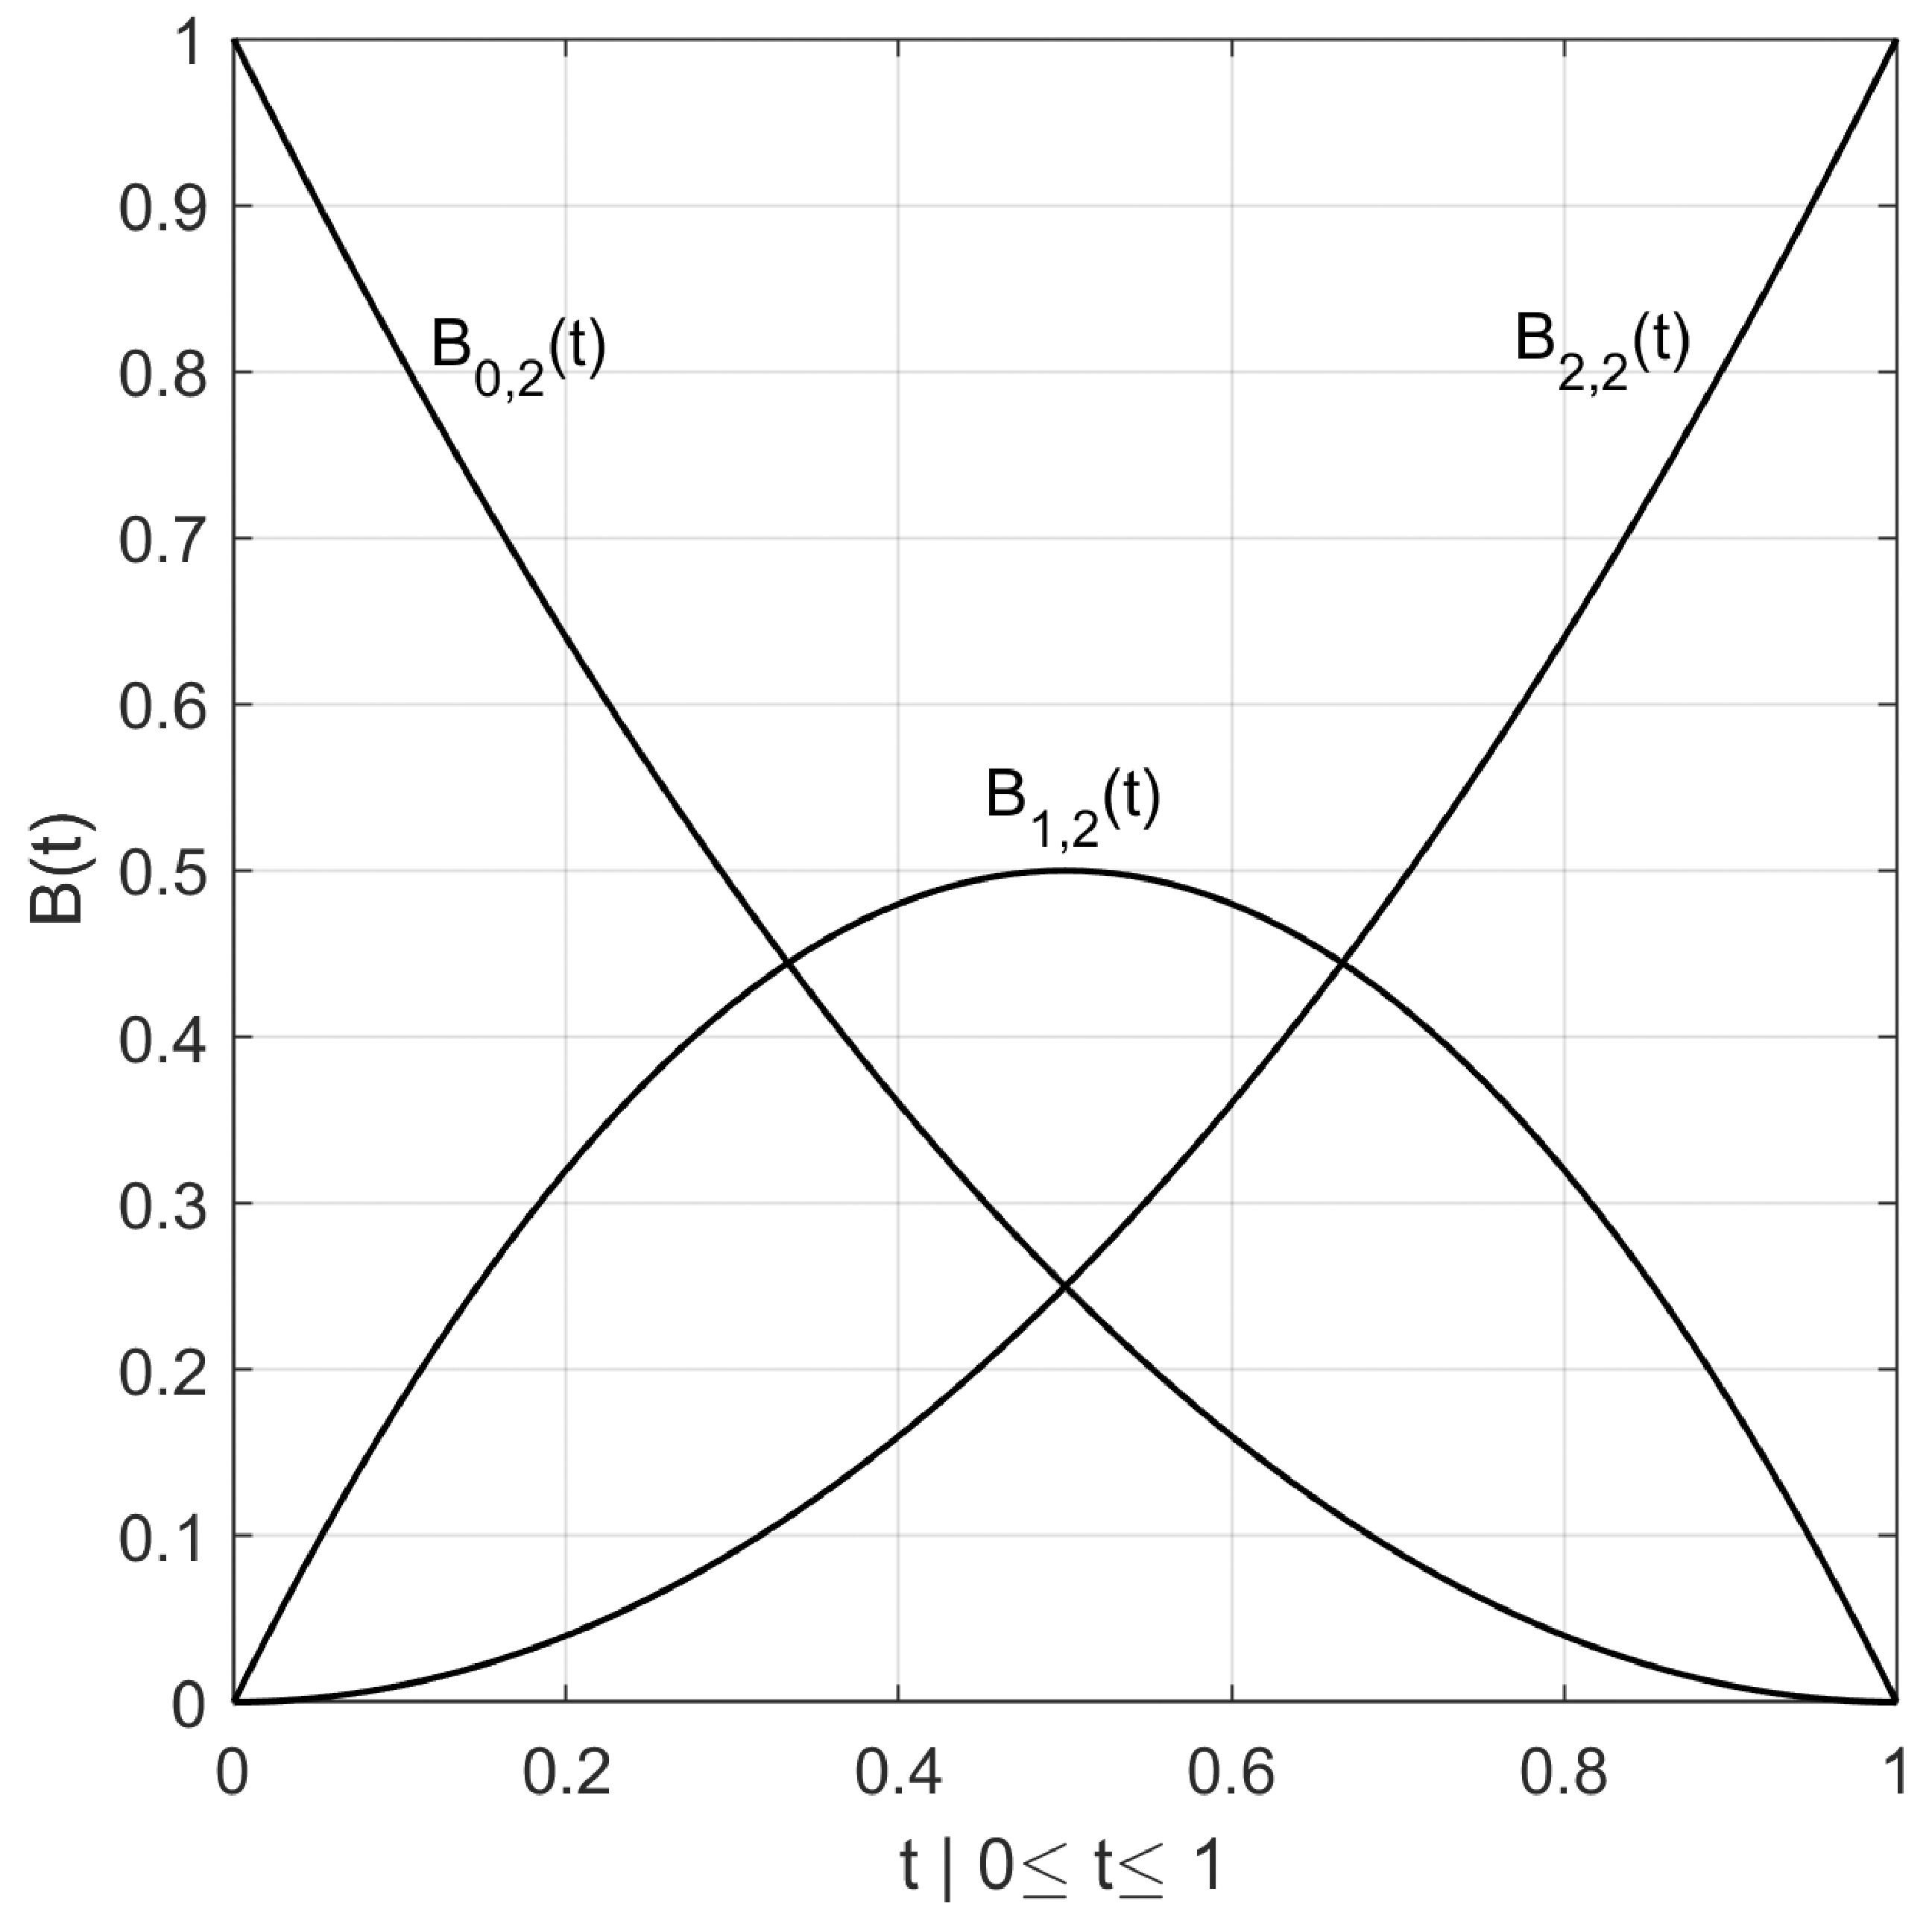
\includegraphics[width=7cm]{bezierquadric.eps}
  \caption{2$^{nd }$ degree Bernstain polynomials.}
  \label{figure02}
\end{figure}




\begin{thebibliography}{00}

%------------------------------------------------------------------------------------------------------------
\bibitem [Atlasus (2018)] {32}    Atlasus, http://atlasus.com.tr/Atlas/UAV   (Access 18.12.2018)

\bibitem [Azhari \& et al (2018)] {30}   Azhari, F., Heidarpour, A., \& Zhao, X.L. (2018). On the use of Bernstain-Bezier functions for modelling the post-fire stress-strain relationship of ultra-high strength steel (Grade 1200). \emph{Engineering Structures}. 175, 605-616.

\bibitem [Bergen \&  Ross (2012)] {20}  Bergen, S., \& Ross, J.R. (2009). Automatic and interactive evolution of vector graphics images with genetic algorithms. \emph{The Visual Computer}, 28, 35-45.

\bibitem [Besdok, Civicioglu, \&  Alci (2004)] {3}  Besdok, E., Civicioglu,  P., \& Alc\i, M. (2004). Impulsive noise suppression from highly corrupted images by using resilient neural networks. \emph{Lecture Notes in Artificial Intelligence}, 3070, 670-675.

\bibitem [Brest et al (2006)] {4}  Brest, J., Greiner, S., Boskovic, B., Mernik, M., \& Zumer V. (2006). Self-adapting control parameters in differential evolution: a comparative study on numerical benchmark problems. \emph{IEEE Transactions on Evolutionary Computation}, 10, 646-657.

\bibitem[Chen, \& et al (2017)] {25} Chen, J.,  Zheng, J.,  Wu, P.,  et al. (2017). Dynamic particle swarm optimizer with escaping prey for solving constrained non-convex and piecewise optimization problems.  \emph{Expert Systems with Applications},  86, 208-223.

\bibitem [Chernikov, \&  Chrisochoides (2012)] {23}  Chernikov, A.N. \&  Chrisochoides, N.P. (2012).  Generalized Insertion Region Guides For Delaunay Mesh Refinement,  \emph{SIAM Journal On Scientific Computing},  34,  A1333-A1350.

\bibitem [Civicioglu (2013{a})] {5} Civicioglu, P. (2013,a). Backtracking search optimization algorithm for numerical optimization problems. \emph{Applied Mathematics and Computation}, 219,  8121-8144.

\bibitem [Civicioglu (2012)] {6}  Civicioglu,  P. (2012). Transforming geocentric cartesian coordinates to geodetic coordinates by using differential search algorithm. \emph{Computers \& Geosciences},  46,  229-247.

\bibitem [Civicioglu (2013{b})] {7} Civicioglu, P. (2013,b). Artificial cooperative search algorithm for numerical optimization problems. \emph{Information Sciences}, 229 - 58-76.

\bibitem [Civicioglu, \&  Alci (2004)] {8} Civicioglu, P., \& Alci M. (2004). Impulsive noise suppression from highly distorted images with triangular interpolants. \emph{AEU - International Journal of Electronics and Communications}, 58,  311-318.

\bibitem [Civicioglu, \&  Besdok (2013)] {9}  Civicioglu, P., \& Be\c{s}dok, E. (2013). A conceptual comparison of the cuckoo-search, particle swarm optimization, differential evolution and artificial bee colony algorithms. \emph{Artificial Intelligence Review}, 39, 315-346.

\bibitem [Civicioglu, \&  Besdok (2014)]  {10}  Civicioglu, P., \& Be\c{s}dok E. (2014). Comparative Analysis of the Cuckoo Search Algorithm,  Cuckoo Search and Firefly Algorithm Theory and Applications, Springer, London,  85-113.

\bibitem [Civicioglu, Besdok, \& et al (2018)] {29}   Civicioglu, P., Besdok, E., Gunen, M.A., \& Atasever, U.H. (2018). Weighted differential evolution algorithm for numerical function optimization: a comparative study with cuckoo search, artificial bee colony, adaptive differential evolution, and backtracking search optimization algorithms. \emph{Neural Computing and Applications}. Article online. https://doi.org/10.1007/s00521-018-3822-5  (Access 18.12.2018)

\bibitem [Matlab (2019{a})] {113} The matlab codes of classic benchmark problems (2019). $ https://www.mathworks.com/matlabcentral/fileexchange/69827-bernstain-search-differential-evolution-algorithm?s\textunderscore
tid$=$FX\textunderscore rc2\textunderscore behav$ (last access 23.06.2019)

\bibitem [Matlab (2019{b})] {114} The matlab codes of classic benchmark problems (2019). $https://www.sfu.ca/~ssurjano/optimization.html$ (last access 23.06.2019)

\bibitem [Clerc, \&  Kennedy (2002)] {11}   Clerc, M., \& Kennedy, J. (2002). The particle swarm-explosion, stability, and convergence in a multidimensional complex space. \emph{IEEE Transactions on Evolutionary Computation}, 6, 58-73.

\bibitem [Das, Mullick, \&  Suganthan (2016)] {12}  Das, S., Mullick, S.S., \& Suganthan, P.N. (2016). Recent advances in differential evolution - An updated survey.  \emph{Swarm and Evolutionary Computation}, 27, 1-30.

\bibitem [Derrac, Garca, \&  Molina (2011)] {13} Derrac, J., Garca, S., Molina, D.,  \& Herrera, F. (2011). A practical tutorial on the use of nonparametric statistical tests as a methodology for comparing evolutionary and swarm intelligence algorithms. \emph{Swarm and Evolutionary Computation}, 1 3-18.

\bibitem [Karabo\~{g}a, \&  Basturk B (2007)] {15} Karabo\~{g}a, D., \& Basturk B. (2007). A powerful and efficient algorithm for numerical function optimization: artificial bee colony (ABC) algorithm.  \emph{Journal of Global Optimization}, 39, 459-471.

\bibitem  [Liang,  Qu, \& Suganthan (2013)] {14} Liang, J.J., \& Qu, B.Y., \&  Suganthan,  P.N. (2013). Problem Definitions and Evaluation Criteria for the CEC 2014 Special Session and Competition on Single Objective Real-Parameter Numerical Optimization, Technical Report 201311, Computational Intelligence Laboratory, Zhengzhou University, Zhengzhou, China  and  Technical Report, Nanyang Technological University, Singapore, December 2013.

\bibitem [Liu \& et al. (2018)] {1} Liu, J., \& Zhang, H., \& He, K. \& et al. (2018). Multi-objective particle swarm optimization algorithm based on objective space division for the unequal-area facility layout problem. \emph{Expert Systems with Applications}, 102, 179-192.

\bibitem [Lynn, \& Suganthan (2017)] {16} Lynn, N., \& Suganthan P.N., (2017).Ensemble particle swarm optimizer.  \emph{Applied Soft Computing}, 55, 533-548.

\bibitem [Opara, \& Arabas (2018)]  {111} Opara K,Arabas J (2018). Comparison of mutation strategies in Differential Evolution – A probabilistic perspective, \emph{Swarm and Evolutionary Computation}. 39, 53–69.

\bibitem [Matsumoto,  \&  Nishimura (1998)] {18}  Matsumoto, M., \& Nishimura, T. (1998). Mersenne twister: A 623-dimensionally equidistributed uniform pseudo-random number generator. \emph{ACM Transactions on Modeling and Computer Simulation}, 8, 3-30.

\bibitem [Mathworks (2019)] {28}   Mathworks, Matlab File Exchange, (2019), https://www.mathworks.com/matlabcentral/fileexchange/69819-bernstain-search-differential-evolution-algorithm    (Last access 25.06.2019)

\bibitem[Mlakar, \& et al (2016)] {27}   Mlakar, U., Potocnik, B.,  \& Brest, J., (2016). A hybrid differential evolution for optimal multilevel image thresholding. \emph{Expert Systems with Applications},  65, 221-232.

\bibitem [Mohamed, \& Suganthan (2018)] {17} Mohamed, A.W., \& Suganthan P.N., (2018). Real-parameter unconstrained optimization based on enhanced fitness-adaptive differential evolution algorithm with novel mutation . \emph{Soft Computing}, 22, 3215-3235.

\bibitem [Price, Storn,  \&  Lampinen (2005)] {19}  Price, K.V., Storn, R.,  \& Lampinen, J. (2005). Differential evolution: A practical approach to global optimization. Springer, Berlin, Germany.

\bibitem [\"{O}zsoydan, Bayka\c{s}o\~{g}lu (2019)] {2}  \"{O}zsoydan, F.B., \& Bayka\c{s}o\~{g}lu, A., (2019). Quantum firefly swarms for multimodal dynamic optimization problems.  \emph{Expert Systems with Applications}, 115, 189-199.

\bibitem [Qin et al (2014)] {21}  Qin, Q., Cheng, S., Zhang, Q., \& et al. (2014). Multiple strategies based orthogonal design particle swarm optimizer for numerical optimization. \emph{Computers \& Operations Research}, 60, 91-110.

\bibitem[Zhang et al (2019)] {112} Zhang, Q., Zou, D., Duan, N., et al. (2019). An adaptive differential evolutionary algorithm incorporating multiple mutation strategies for the economic load dispatch problem. \emph{Applied Soft Computing}, 78, 641-669.

\bibitem [Turef (2018)] {31} Turef, https://epsg.io/5256 (Last access 25.06.2019)

\bibitem [Yang,  \&  Deb (2009)] {22} Yang, X.S., \& Deb, S. (2009). Cuckoo search via levy flights. World Congress on Nature and Biologically Inspired Computing-Nabic\textquoteright 2009, Coimbatore, India, 4, 210-214.

\bibitem [Zhang,  \&  Sanderson (2009)] {24}   Zhang, J., \& Sanderson, A.C. (2009). JADE: Adaptive differential evolution with optional external archive. \emph{IEEE Transactions on Evolutionary Computation},  13, 945-958.

\bibitem[Zhang, \& Zhu (2011) ] {26}  Zhang, W.B., \&  Zhu, G.Y. (2011). Comparison and application of four versions of particle swarm optimization algorithms in the sequence optimization. \emph{Expert Systems with Applications},Volume: 38   Issue: 7   Pages: 8858-8864   Published: JUL 2011

\bibitem[Badea, (2011) ] {40} Badea, C. Bernstein Polynomials and Operator Theory. \emph{Results. Math}. (2009) 53: 229. https://doi.org/10.1007/s00025-008-0333-1

\end{thebibliography}

 \end{document}
